\documentclass[tikz,border=8pt]{standalone}
\usepackage[T1]{fontenc}
\usepackage{lmodern}
\usepackage{xcolor}
\usetikzlibrary{arrows.meta,positioning,fit,calc,backgrounds}
\pgfdeclarelayer{background}
\pgfsetlayers{background,main}

\definecolor{blue}{HTML}{1D4ED8}
\definecolor{teal}{HTML}{0F766E}
\definecolor{green}{HTML}{15803D}
\definecolor{orange}{HTML}{C2410C}
\definecolor{violet}{HTML}{7C3AED}
\definecolor{red}{HTML}{B91C1C}
\definecolor{slate}{HTML}{475569}
\definecolor{line}{HTML}{64748B}
\definecolor{softblue}{HTML}{EFF6FF}
\definecolor{softteal}{HTML}{ECFDF5}
\definecolor{softgreen}{HTML}{F0FDF4}
\definecolor{softviolet}{HTML}{F5F3FF}
\definecolor{softred}{HTML}{FEF2F2}
\definecolor{softgray}{HTML}{F8FAFC}

\newcommand{\subtext}[1]{{\sffamily\scriptsize\color{slate}#1}}
\newcommand{\itemtext}[1]{{\sffamily\footnotesize\color{slate}#1}}

\tikzset{
  font=\sffamily,
  block/.style={
    draw=line,
    rounded corners=2pt,
    fill=white,
    align=center,
    minimum height=12mm,
    text width=36mm,
    inner sep=5pt
  },
  module/.style={
    block,
    minimum height=26mm,
    text width=43mm
  },
  smallmodule/.style={
    block,
    minimum height=22mm,
    text width=38mm
  },
  lane/.style={
    draw=line,
    rounded corners=4pt,
    fill=softgray,
    inner sep=7pt
  },
  arrow/.style={
    -{Latex[length=2.5mm]},
    draw=line,
    line width=0.65pt
  },
  mainarrow/.style={
    -{Latex[length=2.8mm]},
    draw=blue,
    line width=0.9pt
  },
  feedback/.style={
    -{Latex[length=2.4mm]},
    draw=violet,
    dashed,
    line width=0.75pt
  },
  metricarrow/.style={
    -{Latex[length=2.2mm]},
    draw=red,
    dotted,
    line width=0.8pt
  },
  title/.style={
    font=\sffamily\footnotesize\bfseries,
    text=slate,
    anchor=west
  }
}

\begin{document}
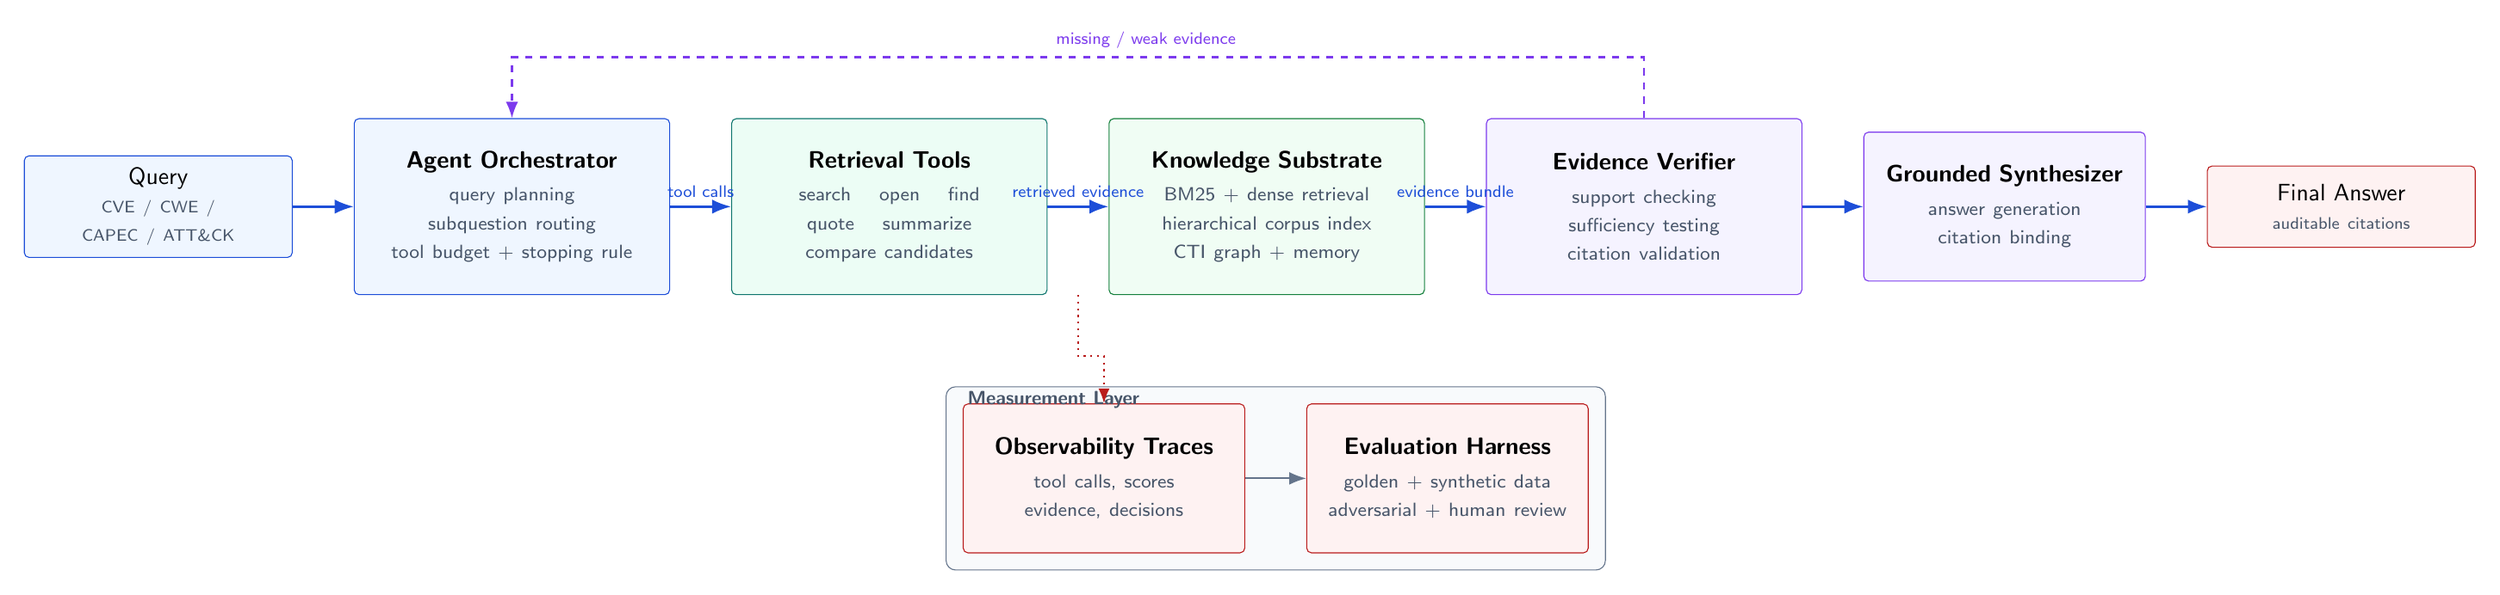
\begin{tikzpicture}[node distance=10mm and 9mm]

% Main pipeline.  Keep this row simple: the paper should read left-to-right.
\node[block, fill=softblue, draw=blue] (query)
  {Query\\\subtext{CVE / CWE / CAPEC / ATT\&CK}};

\node[module, fill=softblue, draw=blue, right=of query] (agent)
  {\textbf{Agent Orchestrator}\\[2pt]
   \itemtext{query planning}\\
   \itemtext{subquestion routing}\\
   \itemtext{tool budget + stopping rule}};

\node[module, fill=softteal, draw=teal, right=of agent] (tools)
  {\textbf{Retrieval Tools}\\[2pt]
   \itemtext{search \quad open \quad find}\\
   \itemtext{quote \quad summarize}\\
   \itemtext{compare candidates}};

\node[module, fill=softgreen, draw=green, right=of tools] (knowledge)
  {\textbf{Knowledge Substrate}\\[2pt]
   \itemtext{BM25 + dense retrieval}\\
   \itemtext{hierarchical corpus index}\\
   \itemtext{CTI graph + memory}};

\node[module, fill=softviolet, draw=violet, right=of knowledge] (verify)
  {\textbf{Evidence Verifier}\\[2pt]
   \itemtext{support checking}\\
   \itemtext{sufficiency testing}\\
   \itemtext{citation validation}};

\node[smallmodule, fill=softviolet, draw=violet, right=of verify] (synth)
  {\textbf{Grounded Synthesizer}\\[2pt]
   \itemtext{answer generation}\\
   \itemtext{citation binding}};

\node[block, fill=softred, draw=red, right=of synth] (answer)
  {Final Answer\\\subtext{auditable citations}};

\draw[mainarrow] (query.east) -- (agent.west);
\draw[mainarrow] (agent.east) -- node[above, font=\sffamily\scriptsize, text=blue] {tool calls} (tools.west);
\draw[mainarrow] (tools.east) -- node[above, font=\sffamily\scriptsize, text=blue] {retrieved evidence} (knowledge.west);
\draw[mainarrow] (knowledge.east) -- node[above, font=\sffamily\scriptsize, text=blue] {evidence bundle} (verify.west);
\draw[mainarrow] (verify.east) -- (synth.west);
\draw[mainarrow] (synth.east) -- (answer.west);

% One feedback loop, placed above the pipeline to avoid crossing the data path.
\draw[feedback] (verify.north) -- ++(0,9mm) -|
  node[pos=0.22, above, font=\sffamily\scriptsize, text=violet]
  {missing / weak evidence}
  (agent.north);

% Measurement sidecar. It observes the whole run without becoming part of the data flow.
\node[smallmodule, fill=softred, draw=red, below=16mm of knowledge, xshift=-24mm] (trace)
  {\textbf{Observability Traces}\\[2pt]
   \itemtext{tool calls, scores}\\
   \itemtext{evidence, decisions}};
\node[smallmodule, fill=softred, draw=red, right=of trace] (eval)
  {\textbf{Evaluation Harness}\\[2pt]
   \itemtext{golden + synthetic data}\\
   \itemtext{adversarial + human review}};

\begin{pgfonlayer}{background}
\node[lane, fit=(trace)(eval)] (measurement) {};
\end{pgfonlayer}
\node[title] at ($(measurement.north west)+(2mm,-2mm)$) {Measurement Layer};

\draw[arrow] (trace.east) -- (eval.west);
\draw[metricarrow] ($(agent.south)!0.5!(verify.south)$) -- ++(0,-9mm) -| (trace.north);

\end{tikzpicture}
\end{document}
